% Regular polytopes realised over rings, after Grothendieck's notes (folders 70, 72, 78, 86) — standalone article for Hexagon.
% pdfLaTeX. Compile: latexmk -pdf article.tex (or tectonic -X compile article.tex).
\documentclass[11pt,a4paper]{amsart}
\usepackage[T1]{fontenc}
\usepackage[utf8]{inputenc}
\usepackage{lmodern,microtype,amssymb,mathtools,enumitem,booktabs}
\usepackage[margin=2.7cm]{geometry}
\usepackage{tikz}
\usetikzlibrary{calc}
\usepackage[hidelinks]{hyperref}
\usepackage{xurl}
\emergencystretch=3em

\newtheorem{theorem}{Theorem}[section]
\newtheorem{proposition}[theorem]{Proposition}
\newtheorem{lemma}[theorem]{Lemma}
\newtheorem{corollary}[theorem]{Corollary}
\theoremstyle{definition}
\newtheorem{definition}[theorem]{Definition}
\theoremstyle{remark}
\newtheorem{remark}[theorem]{Remark}
\newtheorem{example}[theorem]{Example}

\newcommand{\Z}{\mathbb Z}
\newcommand{\F}{\mathbb F}
\newcommand{\Q}{\mathbb Q}
\newcommand{\R}{\mathbb R}
\newcommand{\id}{\mathrm{id}}
\newcommand{\Alt}{\operatorname{Alt}}
\newcommand{\fac}[1]{\href{https://grothendieck.umontpellier.fr/#1.pdf}{folder~#1}}

\title[Regular polytopes over rings]{Regular polytopes realised over arbitrary rings,\\ after Grothendieck's working notes}
\author{Michel Hua}
\address{Commutator, Paris, France}
\email{michel@commutator.io}
\thanks{ORCID 0009-0002-8304-0683.}
\date{7 November 2026}
\subjclass[2020]{51M20; 20F55, 51E15, 52B15, 11B39}
\keywords{regular polytopes, reflection groups over rings, icosahedron, affinely regular polygons, Chebyshev polynomials, hemi-icosahedron, Lean}

\begin{document}
\begin{abstract}
In the \emph{Esquisse d'un programme} Grothendieck announced that the regular polytopes make sense over any field, and even over any base ring, through universal formulae in a few parameters. Four folders of his working notes, kept at the University of Montpellier and dating from the late 1970s, contain the computations behind that announcement. We state and prove the main results they contain, completed or corrected where the pages are incomplete. Over any commutative ring, a regular polygon closes after $n$ steps exactly when a Chebyshev-type polynomial $F_n$ vanishes at its invariant, and in characteristic $p$ there are regular $2p$-gons whose vertices lie on two parallel lines. In any dimension, the rotation $\sigma_k\sigma_{k+1}$ of the universal realisation by reflections satisfies $(t-1)(t^2-\alpha_k t+1) = 0$, and its order is $3$, $4$ or $5$ exactly when $\alpha_k = -1$, $0$ or $\alpha_k^2 + \alpha_k = 1$, over every nonzero ring. Realisations by pseudo-reflections with a pinned start vector are classified over any ring by $2n+1$ parameters, with automorphism group $\mathbb G_m \times \mathcal U_\rho$, where $\mathcal U_\rho$ deforms $\mathbb G_m$ into $\mathbb G_a$. The icosahedron written over $\mathbb Z[\alpha]/(\alpha^2+\alpha-1)$ stays faithful over every nonzero ring, characteristics $2$ and $5$ included. Its circumscribed quadric is smooth whenever $5$ is invertible and, over a field, singular only in characteristic $5$, where it becomes a cone whose six vertex directions fill a conic of $\mathbb P^2(\mathbb F_5)$. Finally, the combinatorial icosahedron carries five distinguished triples of edge directions on which its group acts through $\Alt_5$, and the hemi-icosahedron is rebuilt from an oriented set of five elements. All statements are formalised in Lean.
\end{abstract}

\maketitle

\section{Introduction}

In the \emph{Esquisse d'un programme} \cite[\S4]{esquisse}, written in 1984, Grothendieck describes a project from the late 1970s: to realise the regular polyhedra, and more generally the regular maps and polytopes \cite{coxeter1973,mcmullenschulte2002}, over any field and even over any base ring, without lengths or angles, by universal formulae in a few parameters, the doubles of the cosines of the fundamental angles. He adds that the icosahedron specialised to a finite field remains an icosahedron, and that the characteristics $2$ and $5$ are the most singular. Ji \cite{ji2023} has recently reconstructed part of this programme from the \emph{Esquisse} alone, and observes that his own formulae for the icosahedron are undefined in characteristics $2$ and $5$.

The University of Montpellier holds the mathematical papers that Grothendieck left to Jean Malgoire and publishes their facsimiles. Four of its folders contain the computations behind the passage of the \emph{Esquisse}:
\begin{itemize}[leftmargin=1.5em]
\item \fac{70}, \emph{Réalisations géométriques de structures combinatoires (vieilles rédactions)}: the universal formulae and the icosahedron over $\Z[\alpha]$;
\item \fac{72}, \emph{Polyèdres réguliers et hyperpolyèdres réguliers (calculs en dimension quelconque)}, dated from 1978 by the inventory: realisations by pseudo-reflections over a base;
\item \fac{78}, \emph{Polygones réguliers et polynômes cyclotomiques}, dated from 1977: regular polygons over a ring;
\item \fac{86}, \emph{Polyèdres réguliers}: the icosahedron as a combinatorial object.
\end{itemize}
This paper states and proves the main results of these folders. The statements are attributed to Grothendieck when the page states them, with the page; otherwise they are said to be \emph{after} the page, in a form the edition completed or corrected, and each such change is described. The proofs are ours, except where we follow the page and say so. Every result is formalised in Lean~4 with Mathlib (Section~\ref{sec:lean}).

\subsection*{Summary}
Section~\ref{sec:poly} treats polygons: the closure criterion $u_\alpha^n = 1 \iff F_n(\alpha) = 0$ over any ring (Theorem~\ref{thm:closure}), and the regular $2p$-gons on two parallel lines in characteristic $p$ (Proposition~\ref{prop:strip}). Section~\ref{sec:univ} treats the universal formulae in any dimension and the order criterion (Theorems~\ref{thm:univ} and~\ref{thm:anyp}). Section~\ref{sec:pinned} classifies pinned realisations by pseudo-reflections over a ring and computes their automorphisms (Theorems~\ref{thm:AB}, \ref{thm:classif}, \ref{thm:aut}), and lists the invariant subspaces over a field (Theorem~\ref{thm:inv}). Section~\ref{sec:ico} proves that the icosahedron over $\Z[\alpha]$ is faithful over every nonzero ring and studies its quadric and its reduction modulo~$5$ (Theorems~\ref{thm:faithful}, \ref{thm:quadric}, \ref{thm:mod5}). Section~\ref{sec:comb} treats the combinatorial icosahedron and the hemi-icosahedron (Theorems~\ref{thm:triedres} and~\ref{thm:hemi}).

\section{Regular polygons over a ring}\label{sec:poly}

Folder~78 looks for a definition of the regular polygon in an affine plane over an arbitrary field or ring, without lengths or angles: an $n$-gon each of whose combinatorial automorphisms extends uniquely to an affinity. In the frame of three consecutive vertices $(s_0, s_1, s_{-1})$, pages~81 to~85 reduce such a polygon, when it is \emph{proper}, to one parameter $\alpha$, its numerical invariant, and the rotation becomes
\[
u_\alpha(x, y) = (1 - y + \alpha x,\ x),
\]
a bijection of $k^2$ with inverse $(x, y) \mapsto (y, 1 - x + \alpha y)$. Let $k$ be a commutative ring, $\alpha \in k$, and $s_n = u_\alpha^n(0,0)$ for $n \in \Z$.

Let $S_m \in \Z[U]$ be the renormalised Chebyshev polynomials of the second kind: $S_0 = 1$, $S_1 = U$, $S_{m+1} = US_m - S_{m-1}$ for all $m \in \Z$, so that $S_{-1} = 0$. Following page~109, put
\[
F_{2m} = S_{m-1}, \qquad F_{2m+1} = S_m + S_{m-1} \qquad (m \in \Z),
\]
so $F_0 = 0$, $F_1 = F_2 = 1$, $F_3 = U + 1$, $F_4 = U$, $F_5 = U^2 + U - 1$, $F_6 = U^2 - 1$, and $F_{-n} = -F_n$. For $t$ invertible with inverse $t'$ and $m \ge 0$, one has $F_{2m+2}(t + t')(t^2 - 1)t^m = t^{2m+2} - 1$ and $F_{2m+1}(t + t')(t - 1)t^m = t^{2m+1} - 1$, by induction from the recurrence $F_{n+4} = UF_{n+2} - F_n$.

\begin{theorem}[Grothendieck, \fac{78}, pp.~109--113]\label{thm:closure}
\leavevmode
\begin{enumerate}
\item For every $n \in \Z$, in $\Z[U]$,
\[
F_nF_{n+1} - UF_{n-1}F_n + F_{n-2}F_{n-1} = 1;
\]
equivalently $A_nF_{n-1} + F_nF_{n+1} = 1$ with $A_n = F_{n-2} - UF_n$. In particular $F_{n-1}$ and $F_{n+1}$ are coprime.
\item For every $n \in \Z$ and $(x, y) \in k^2$, with $X_n = (F_nF_{n+1})(\alpha)$,
\[
u_\alpha^n(x, y) = (1 - x - y)\,s_n + x\,s_{n+1} + y\,s_{n-1}, \qquad s_n = (X_n, X_{n-1}).
\]
\item For every $n \in \Z$ the following are equivalent: (a) $u_\alpha^n = \id$; (b) $s_n = s_0$; (c) $u_\alpha^n$ fixes some vertex $s_i$; (d) $F_n(\alpha) = 0$.
\end{enumerate}
\end{theorem}

\begin{proof}
(1) For $n = 2m$, the four polynomials are $S_{m-1}$, $S_m + S_{m-1}$, $S_{m-1} + S_{m-2}$, $S_{m-2}$; replacing $S_m$ by $US_{m-1} - S_{m-2}$, the left-hand side becomes $Q_{m-1}$, where $Q_m = S_m^2 - US_mS_{m-1} + S_{m-1}^2$. The odd case gives $Q_m$ in the same way. Now $Q_{m+1} = S_{m+1}(S_{m+1} - US_m) + S_m^2 = S_m^2 - S_{m+1}S_{m-1} = Q_m$, and $Q_0 = 1$: this is the Cassini identity of the $S_m$.

(2) The identity at rank $n+1$, evaluated at $\alpha$, gives $X_{n+1} = \alpha X_n - X_{n-1} + 1$. Call $V_n(x,y)$ the right-hand side. Then $V_0 = \id$, since $X_0 = X_{-1} = 0$ and $X_1 = X_{-2} = 1$, and $u_\alpha \circ V_n = V_{n+1}$, because the weights $1 - x - y$, $x$, $y$ sum to $1$ and each $1 - X_{j-1} + \alpha X_j$ equals $X_{j+1}$. Induct upwards, and downwards since $u_\alpha$ is bijective.

(3) (a)$\Rightarrow$(b) is clear. (d)$\Rightarrow$(a): if $F_n(\alpha) = 0$, then $X_n = X_{n-1} = 0$, hence $X_{n+1} = X_{n-2} = 1$, and (2) gives $u_\alpha^n = \id$. (b)$\Rightarrow$(d): if $(F_nF_{n+1})(\alpha) = (F_{n-1}F_n)(\alpha) = 0$, multiply the identity of (1) at $\alpha$ by $F_n(\alpha)$:
\[
F_n(\alpha) = F_n(\alpha)\,(F_nF_{n+1})(\alpha) + \bigl(F_{n-2}(\alpha) - \alpha F_n(\alpha)\bigr)(F_{n-1}F_n)(\alpha) = 0.
\]
(b)$\Leftrightarrow$(c): $u_\alpha^n(s_i) = u_\alpha^i(s_n)$ and $u_\alpha^i$ is injective.
\end{proof}

The criterion holds over every commutative ring, zero divisors included, because the converse uses only the Bézout relation of (1) and no factorisation. Over a field, Bachmann and Schmidt gave a criterion of the same kind for the linear circular system $v_{i-1} + cv_i + v_{i+1} = 0$ ($i$ modulo $n$), as recalled by Korchmáros and Sz\H{o}nyi \cite[(3.4)]{korchmarosszonyi2008}: it has a nontrivial solution iff $c = \pm2$ or $x^2 - cx + 1$ divides $x^n - 1$. Fisher and Jamison \cite{fisherjamison1998} relate the diagonals of affinely regular polygons over a field to Chebyshev polynomials of the second kind. In terms of the Lucas sequence $U_m = U_m(\alpha, 1)$ \cite{lucas1878}, $F_{2m}(\alpha) = U_m$ and $F_{2m+1}(\alpha) = U_{m+1} + U_m$. On page~113 the first Bézout coefficient is written $F_{n-2} - UF_{n-1}$, which fails already for $n = 4$; the correct coefficient is $A_n$ above. The page also concludes ``$F_n(\alpha) = 1$'' on page~112, where $F_n(\alpha) = 0$ is meant. An affinity of $k^2$ is determined by its values at $s_0 = (0,0)$, $s_1 = (1,0)$, $s_{-1} = (0,1)$, so a combinatorial automorphism of the polygon extends in at most one way; together with $\sigma_1 u_\alpha \sigma_1 = u_\alpha^{-1}$, where $\sigma_1(x,y) = (y,x)$, the dihedral group acts on the vertices. The quadratic function $f_\alpha(x,y) = x^2 - x + y^2 - y - \alpha xy$ of page~96 is $u_\alpha$-invariant and vanishes at every vertex.

\subsection*{Polygons on two parallel lines}
A \emph{characteristic} of a nonzero ring $k$ is an integer $p \ge 0$ such that $m \in \Z$ maps to $0$ in $k$ exactly when $p \mid m$. Pages~84--85 and~94--99 describe two polygons in characteristic $p$ whose vertices lie alternately on two parallel lines: the one with invariant $\alpha = -2$, and the \emph{improper} one, with rotation $v(x,y) = (1 - y, -x)$. Put $t_n = v^n(0,0)$.

\begin{proposition}[after \fac{78}, pp.~84, 85, 94--99]\label{prop:strip}
Let $k$ be a nonzero ring of characteristic $p$.
\begin{enumerate}
\item $s_{2m} = (-m, m)$ and $s_{2m+1} = (1+m, -m)$ for $\alpha = -2$: the even vertices lie on $x + y = 0$, the odd ones on $x + y = 1$, and $f_{-2} = (x+y)(x+y-1)$.
\item $u_{-2}^n = \id$ iff $2p \mid n$, iff $F_n(-2) = 0$; so $u_{-2}$ has order $2p$, and $s_n = s_m$ iff $2p \mid n - m$.
\item Three consecutive vertices are never collinear: $\det(s_{n+1} - s_n, s_{n-1} - s_n) = 1$.
\item For the improper polygon, $v^{2m}$ is the translation by $m(1,-1)$, $t_{2m} = (m, -m)$, $t_{2m+1} = (m+1, -m)$; $v$ has order $2p$, three consecutive vertices are not collinear, $\sigma_1 v\sigma_1 = v^{-1}$, and the linear part of $v$ has determinant $-1$, while that of $u_{-2}$ has determinant $1$.
\end{enumerate}
\end{proposition}

\begin{proof}
(1) By induction both ways: $u_{-2}(-m, m) = (1+m, -m)$ and $u_{-2}(1+m, -m) = (-(m+1), m+1)$. (2) $s_{2m} = (0,0)$ iff $m = 0$ in $k$, iff $p \mid m$; and $s_{2m+1} = (0,0)$ would force $1 = 0$. Theorem~\ref{thm:closure} gives the rest. (3) For $n = 2m$ the two vectors are $(1+2m, -2m)$ and $(2m, 1-2m)$, of determinant $1$; the odd case is similar. (4) By induction, $v^{2m}(x,y) = (x+m, y-m)$ and $v^{2m+1}(x,y) = (1-y+m, -x-m)$, and one argues as in (2).
\end{proof}

No primality or parity of $p$ is needed. For $p = 2$, $\alpha = -2 = 0$ and one recovers the square; for $p = 0$ both rotations have infinite order and the vertices form the two staircase $\infty$-gons of page~85. The two polygons have the same vertex set, $s_{2m+1} = t_{2m+1}$ and $s_{2m} = t_{-2m}$: the first zigzags along the two lines in opposite directions, the second climbs them in the same direction (Figure~\ref{fig:strip}). For $p \ge 3$ each line carries $p$ vertices, so these polygons are degenerate in the sense of Korchmáros and Sz\H{o}nyi (three vertices are collinear, though never three consecutive ones). Their survey is consistent with this: over a field, every non-degenerate affinely regular polygon lies on an irreducible conic \cite[Lemma~2.2]{korchmarosszonyi2008}, the classification \cite[Th.~2.1 and~2.3]{korchmarosszonyi2008} lists ellipses, hyperbolas and, in characteristic $p$, parabolas carrying $p$-gons, and the case $c = -2$ of the circular system is discussed there for $n$ prime to the characteristic, where the even vertices coincide and so do the odd ones. We have not found the two-line $2p$-gons in that survey. Here the invariant conic $f_{-2} = 0$ is the pair of lines.

\begin{figure}[ht]
\centering
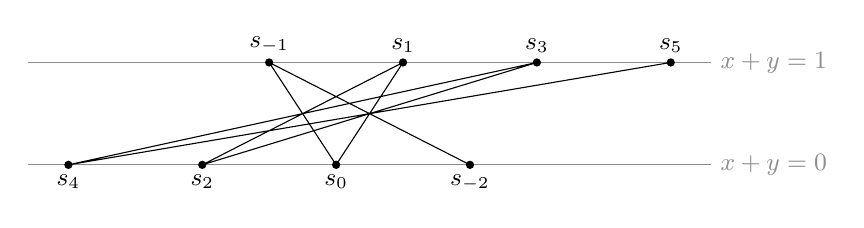
\begin{tikzpicture}[x=0.85cm, y=1.3cm, every node/.style={font=\small}]
\draw[black!45] (-4.6,0) -- (5.6,0) node[right] {$x + y = 0$};
\draw[black!45] (-4.6,1) -- (5.6,1) node[right] {$x + y = 1$};
\coordinate (a) at (2,0); \coordinate (b) at (-1,1); \coordinate (c) at (0,0); \coordinate (d) at (1,1);
\coordinate (e) at (-2,0); \coordinate (f) at (3,1); \coordinate (g) at (-4,0); \coordinate (h) at (5,1);
\draw (a)--(b)--(c)--(d)--(e)--(f)--(g)--(h);
\foreach \p in {a,b,c,d,e,f,g,h} \fill (\p) circle (1.5pt);
\node[below] at (a) {$s_{-2}$}; \node[above] at (b) {$s_{-1}$}; \node[below] at (c) {$s_0$}; \node[above] at (d) {$s_1$};
\node[below] at (e) {$s_2$}; \node[above] at (f) {$s_3$}; \node[below] at (g) {$s_4$}; \node[above] at (h) {$s_5$};
\end{tikzpicture}
\caption{The polygon of invariant $\alpha = -2$, drawn over $\Q$ in the coordinates $(x - y, x + y)$. Over $\Q$ it does not close; in characteristic $p$, $s_{n+2p} = s_n$ and it is a $2p$-gon.}\label{fig:strip}
\end{figure}

\section{The universal formulae in any dimension}\label{sec:univ}

Pages~9 to~25 of folder~70 write every regular affine realisation by reflections of the polytope $\{p_1, \dots, p_n\}$ in the frame of its vertices $(s_0, \dots, s_{n+1})$, with $n$ parameters $\alpha_0, \dots, \alpha_{n-1}$. Let $R$ be a commutative ring and $\alpha_0, \dots, \alpha_{n-1} \in R$. In barycentric coordinates $(t_0, \dots, t_{n+1})$ with respect to this frame, put
\[
\ell_i = t_i - t_{i+1} + (1 + \alpha_i)(t_{i+2} + \dots + t_{n+1}), \qquad \sigma_i = \id + \ell_i \otimes (s_{i+1} - s_i) \quad (0 \le i \le n),
\]
and $w_i = s_{i+1} - s_i$ (for $i = n$ the coefficient $\alpha_n$ does not occur).

\begin{theorem}[after \fac{70}, pp.~19, 23--25 and~67]\label{thm:univ}
Let $n \ge 1$.
\begin{enumerate}
\item For all $\alpha_i$: $\sigma_i^2 = 1$; $\sigma_i\sigma_j = \sigma_j\sigma_i$ for $i + 2 \le j \le n$; $\sigma_i$ preserves $t_0 + \dots + t_{n+1}$; $\sigma_is_i = s_{i+1}$, $\sigma_is_j = s_j$ for $j < i$, and $\sigma_is_j = s_j + (1 + \alpha_i)w_i$ for $i + 2 \le j \le n+1$.
\item For $k \le n - 1$ the image of $\sigma_k\sigma_{k+1} - 1$ lies in the plane $W = \langle w_k, w_{k+1}\rangle$, and $(t - 1)(t^2 - \alpha_kt + 1)$ annihilates $\rho = \sigma_k\sigma_{k+1}$.
\item If $R \ne 0$, $\rho$ has order exactly $3$, $4$ or $5$ iff, respectively, $\alpha_k = -1$, $\alpha_k = 0$, or $\alpha_k^2 + \alpha_k - 1 = 0$.
\end{enumerate}
\end{theorem}

\begin{proof}
(1) $\ell_i(w_i) = -2$ gives $\ell_i(\sigma_ix) = -\ell_i(x)$, hence $\sigma_i^2 = 1$. For $i + 2 \le j \le n$, $\ell_i(w_j) = 0 = \ell_j(w_i)$, so both products are $x \mapsto x + \ell_i(x)w_i + \ell_j(x)w_j$. The rest is read on the values $\ell_i(s_j)$.

(2) Since $\ell_{k+1}(w_k) = 1$ and $\ell_k(w_{k+1}) = 2 + \alpha_k$,
\[
\rho w_k = (1 + \alpha_k)w_k + w_{k+1}, \qquad \rho w_{k+1} = -(2 + \alpha_k)w_k - w_{k+1},
\]
so $\rho$ has trace $\alpha_k$ and determinant $1$ on $W$, which contains the image of $\rho - 1$.

(3) Write $\rho^m x = x + \sum_{j<m}\rho^j(\rho x - x)$. On $W$, $\sum_{j<3}\rho^j = (1 + \alpha_k)\rho$, $\sum_{j<4}\rho^j = \alpha_k\bigl((1 + \alpha_k)\rho - 1\bigr)$ and $\sum_{j<5}\rho^j = (\alpha_k^2 + \alpha_k - 1)(\alpha_k\rho - 1)$, which vanish under the corresponding hypothesis. Conversely, on $\langle s_k, s_{k+1}, s_{k+2}\rangle$, $\rho(a,b,c) = \bigl(c - (1+\alpha)b,\ a + (1+\alpha)b,\ b\bigr)$ with $\alpha = \alpha_k$, and the iterates of $s_k = (1,0,0)$ are $(0,1,0)$, $(-1-\alpha, 1+\alpha, 1)$, $(-2\alpha - \alpha^2, \alpha + \alpha^2, 1 + \alpha)$, then vectors whose last two coordinates are $(\alpha^3 + \alpha^2 - \alpha, \alpha + \alpha^2)$ and $\bigl((\alpha^2 - 1)P, \alpha P\bigr)$, with $P = \alpha^2 + \alpha - 1$. So $\rho^3s_k = s_k$ forces $1 + \alpha = 0$; $\rho^4s_k = s_k$ forces $\alpha + \alpha^2 = 0 = \alpha^3 + \alpha^2 - \alpha$, hence $\alpha = \alpha(\alpha + \alpha^2) - (\alpha^3 + \alpha^2 - \alpha) = 0$; and $\rho^5s_k = s_k$ forces $P = \alpha\cdot\alpha P - (\alpha^2 - 1)P = 0$. Under each hypothesis, the iterates of order $m < p$ have a coordinate equal to $1$ where $s_k$ has $0$, so $\rho^m \ne 1$ when $R \ne 0$.
\end{proof}

On the affine plane $s_k + W$, which $\rho$ preserves, the linear part of $\rho$ has trace $\alpha_k$ and determinant $1$; over $\R$ it is conjugate to the rotation by $2\pi/p$ when $\alpha_k = 2\cos(2\pi/p)$, and $-1$, $0$, $(\sqrt5 - 1)/2$ give $p = 3, 4, 5$ (Figure~\ref{fig:orders}). The parameters are thus twice the cosines of the rotation angles, which is presumably the sense of the \emph{Esquisse}'s ``doubles of the cosines of the fundamental angles''. Ji's formulae are written in the cosines themselves, and he notes that he could not reconcile them with the doubles \cite[\S2]{ji2023}. The five Platonic solids are $(\alpha_0, \alpha_1) = (-1,-1)$ (tetrahedron), $(0,-1)$ (cube), $(-1,0)$ (octahedron), $(\alpha,-1)$ (dodecahedron) and $(-1,\alpha)$ (icosahedron), with $\alpha^2 + \alpha = 1$; the other root of $\alpha^2 + \alpha - 1$ gives the star polyhedra of page~69.

\begin{figure}[ht]
\centering
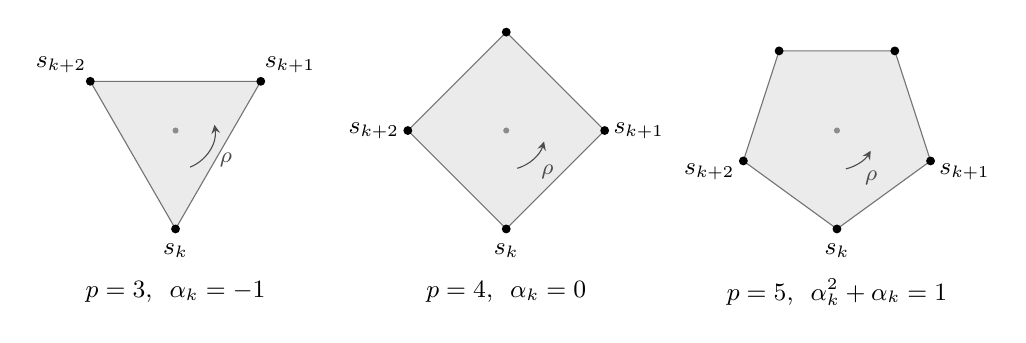
\begin{tikzpicture}[x=1cm, y=1cm, >=stealth, every node/.style={font=\small}]
\foreach \p/\dx/\al in {3/0/{\alpha_k = -1}, 4/4.2/{\alpha_k = 0}, 5/8.4/{\alpha_k^2 + \alpha_k = 1}} {
  \begin{scope}[xshift=\dx cm]
  \pgfmathsetmacro{\stp}{360/\p}
  \pgfmathsetmacro{\anA}{90+\stp}
  \pgfmathsetmacro{\anB}{90-\stp}
  \fill[black!8] (-90:1.25) \foreach \j in {1,...,\p} { -- ({-90+\j*\stp}:1.25) } -- cycle;
  \draw[black!55] (-90:1.25) \foreach \j in {1,...,\p} { -- ({-90+\j*\stp}:1.25) } -- cycle;
  \fill[black!45] (0,0) circle (1.1pt);
  \draw[->, black!70] ({-90+0.18*\stp}:0.5) arc[start angle={-90+0.18*\stp}, end angle={-90+0.82*\stp}, radius=0.5];
  \node[black!70] at ({-90+0.5*\stp}:0.74) {\footnotesize $\rho$};
  \foreach \j in {1,...,\p} \fill ({-90+\j*\stp}:1.25) circle (1.6pt);
  \node[below=2pt] at (-90:1.25) {$s_k$};
  \node[anchor=\anA, inner sep=3pt] at ({-90+\stp}:1.25) {$s_{k+1}$};
  \node[anchor=\anB, inner sep=3pt] at ({-90-\stp}:1.25) {$s_{k+2}$};
  \node at (0,-2.05) {$p = \p$, \ $\al$};
  \end{scope}
}
\end{tikzpicture}
\caption{The orbit of $s_k$ under $\rho = \sigma_k\sigma_{k+1}$ in the affine plane $s_k + W$, over $\R$, in an affine coordinate where the linear part of $\rho$ is a rotation.}\label{fig:orders}
\end{figure}

Page~67 states for $n = 2$, without proof, that $\rho^p = \id$ iff $F_p(\alpha) = 0$. For arbitrary $p$ we have the following form.

\begin{theorem}[after \fac{70}, p.~67]\label{thm:anyp}
Let $n \ge 1$, $k \le n-1$ and $\rho = \sigma_k\sigma_{k+1}$.
\begin{enumerate}
\item If $R \ne 0$, then for every $m \ge 0$, $\rho^m = 1$ iff $\chi = (t-1)(t^2 - \alpha_kt + 1)$ divides $t^m - 1$ in $R[t]$.
\item For $p \ge 3$ let $\Psi_p \in \Z[x]$ be the minimal polynomial of $2\cos(2\pi/p)$, of degree $d$. Then $x^d\Psi_p(x + x^{-1}) = \Phi_p(x)$, the $p$-th cyclotomic polynomial, and $2d = \varphi(p)$.
\item If $R = K$ is a field of characteristic $0$ and $p \ge 3$, then $\rho$ has order exactly $p$ iff $\Psi_p(\alpha_k) = 0$.
\end{enumerate}
\end{theorem}

\begin{proof}
(1) $\chi(\rho) = 0$ by Theorem~\ref{thm:univ}(2). Conversely, if $\rho^m = 1$, the remainder $r = r_0 + r_1t + r_2t^2$ of $t^m - 1$ modulo the monic $\chi$ satisfies $r(\rho)s_k = r_0s_k + r_1s_{k+1} + r_2\bigl(s_{k+2} + (1+\alpha_k)w_k\bigr) = 0$, whence $r_2 = r_1 = r_0 = 0$: the vector $s_k$ is cyclic. (2) $T = x^d\Psi_p(x + x^{-1})$ is an integer polynomial of degree at most $2d$ and constant term $1$, vanishing at $\zeta = e^{2i\pi/p}$, so $\Phi_p \mid T$; and $\deg\Phi_p = [\Q(\zeta):\Q(\cos(2\pi/p))]\,d \ge 2d$, since $\Q(\cos(2\pi/p))$ is real and $\zeta$ is not. Hence $T = c\,\Phi_p$ with $c$ constant, and $c = 1$ since both have constant term $1$. (3) Let $\zeta$ be a root of $t^2 - \alpha_kt + 1$ in an algebraic closure; $\alpha_k = \zeta + \zeta^{-1}$. In characteristic $0$, $t^m - 1$ has simple roots for $m \ge 1$, so by (1) $\rho^m = 1$ iff $\zeta^m = 1$ and $\zeta^2 \ne 1$ (the roots $1$, $\zeta$, $\zeta^{-1}$ of $\chi$ must be distinct); thus $\rho$ has order $p$ iff $\zeta$ is a primitive $p$-th root of unity, iff $\Phi_p(\zeta) = 0$, iff $\Psi_p(\alpha_k) = 0$ by (2).
\end{proof}

For $p = 3, 4, 5$, $\Psi_p = x + 1$, $x$, $x^2 + x - 1$, and Theorem~\ref{thm:univ}(3) is the same statement over every nonzero ring. In positive characteristic the criterion for arbitrary $p$ is not proved here.

\section{Pinned realisations by pseudo-reflections over a base}\label{sec:pinned}

Folder~72 studies realisations of the universal regular polytope of rank $n+1$ by pseudo-reflections
\[
\tau_i = \id + a'_i \otimes a_i \qquad (0 \le i \le n)
\]
of a module $E$ over a commutative ring $k$, with $a_i \in E$, $a'_i \in E^\vee$, and non-consecutive $\tau_i$ commuting. Given a start vector $s_0$, put $s_{i+1} = \tau_is_i$ and $\nu_i = \langle s_0, a'_0\rangle\langle a_0, a'_1\rangle\cdots\langle a_{i-1}, a'_i\rangle$. Pages~96 to~100 and~103 compare two sets of conditions; a family is called \emph{free} in the strong sense of page~103 when it is independent and spans a direct summand.
\begin{itemize}[leftmargin=2.5em]
\item[(A)] non-consecutive $\tau_i$ commute, $\tau_is_0 = s_0$ for $1 \le i \le n$, and $(s_0, \dots, s_{n+1})$ is free;
\item[(B)] $\langle a_i, a'_j\rangle = 0$ for $|i - j| \ge 2$, $\langle s_0, a'_i\rangle = 0$ for $1 \le i \le n$, $(s_0, a_0, \dots, a_n)$ is free, and $\nu_n$ is invertible.
\end{itemize}

\begin{theorem}[after \fac{72}, pp.~96--100 and~103]\label{thm:AB}
Over every commutative ring $k$ and for every $k$-module $E$, (A) and (B) are equivalent. For independence alone, (A) does not imply the invertibility of $\nu_n$: over $\Z$, with $n = 0$, $s_0 = e_0$, $a_0 = e_1$, $a'_0 = 2e_0^*$, the family $(s_0, s_1) = (e_0, e_0 + 2e_1)$ is independent and $\nu_0 = 2$. If $(s_0, \dots, s_{n+1})$ is a basis of $E$, then $E$ is free.
\end{theorem}

\begin{proof}[Sketch]
One reduces to the submodule $N$ spanned by the family, in which it is a basis. Under (A), $s_{i+1} - s_i = \langle s_i, a'_i\rangle a_i$, and the coordinate on $s_{i+1}$ of the projection onto $N$ shows that $\langle s_i, a'_i\rangle$ is invertible; so $a_i \in N$, the $\tau_i$ restrict to $N$, and the commutation of $\tau_i$ and $\tau_j$ becomes $\langle a_i, a'_j\rangle = 0$. Under (B), $\langle s_i, a'_i\rangle = \nu_i$, by induction on $i$, since $\langle s_{i-1}, a'_i\rangle = 0$; in both directions the transition matrix between $(s_0, \dots, s_{n+1})$ and $(s_0, a_0, \dots, a_n)$ is triangular with invertible diagonal.
\end{proof}

A realisation satisfying (B) with $E$ free of rank $n+2$ is \emph{pinned} and \emph{normalised} when $\langle s_0, a'_0\rangle = 1$ and $\langle a_{i-1}, a'_i\rangle = 1$. Its invariants are $\mu_i = \langle a_i, a'_i\rangle = \lambda_i - 1$ and $\beta_i = \langle a_{i+1}, a'_i\rangle$, so that $\tau_ia_i = \lambda_ia_i$ and $\tau_ia_{i+1} = a_{i+1} + \beta_ia_i$.

\begin{theorem}[after \fac{72}, p.~13 and pp.~91--100]\label{thm:classif}
A normalised pinned realisation is isomorphic, by a unique isomorphism sending $s_0$ to $e_0$ and conjugating the $\tau_i$, to the coordinate realisation on $k^{n+2}$ with basis $(s_0, a_0, \dots, a_n)$ and parameters $(\mu_i, \beta_i)$. The coordinate realisation satisfies (B) for all parameters, and $\tau_i$ is invertible iff $\lambda_i$ is. A linear map between two normalised realisations that is compatible with $s_0$ and the $\tau_i$ forces their parameters to be equal. Non-degenerate pinned realisations on a free module of rank $n+2$ are thus classified, rigidly, by the $2n+1$ parameters $(\lambda_0, \beta_0, \lambda_1, \dots, \beta_{n-1}, \lambda_n)$, with $\lambda_i \in k^\times$ and $\beta_i \in k$.
\end{theorem}

Over $\R$, for representations of a Coxeter group generated by reflections, the reflections determine their Cartan matrix $(\alpha_i(v_j))$ only up to conjugation by a diagonal matrix \cite[\S3.2]{dgklm2021}. Monson and Schulte reduce the root-lattice representation of a crystallographic Coxeter group modulo an odd prime and ask when the image is the group of an abstract regular polytope \cite{monsonschulte2004}. Theorem~\ref{thm:classif} works over any ring, with pseudo-reflections of arbitrary eigenvalue $\lambda_i$, and the start vector $s_0$ removes the diagonal ambiguity. The count $2n+1$ agrees with the $n + (n+1)$ variables that a footnote of the \emph{Esquisse} announces for the universal pseudo-polyhedron, one additional invariant for each pseudo-reflection \cite[\S4]{esquisse}.

\subsection*{Automorphisms}
In the basis $(s_0, a_0, \dots, a_n)$ let $\pi$ be the first coordinate, and $\tilde c$ the unique vector killed by all the $a'_i$ whose coordinate on $a_n$ is $1$, obtained by back substitution. Put $\rho = \pi(\tilde c)$; for $n = 1$, $\rho = \mu_0\mu_1 - \beta_0$, which is $4 - \beta_0$ for reflections, as on page~41. Page~37 introduces the group $\mathcal U_\rho = \operatorname{Spec}\mathcal O_S[T]_{(1+\rho T)}$ with law $\lambda * \lambda' = \lambda + \lambda' + \rho\lambda\lambda'$, acting by $u_\lambda = \id + \lambda\,\pi\otimes\tilde c$; the theorem of page~38 asserts without proof that $\mathbb G_m \times \mathcal U_\rho \to \operatorname{Aut}(E, (\tau_i))$ is an isomorphism.

\begin{theorem}[after \fac{72}, pp.~37--38, on points]\label{thm:aut}
The $\lambda \in k$ with $1 + \rho\lambda$ invertible form a commutative group $\mathcal U_\rho(k)$; $\lambda \mapsto 1 + \rho\lambda$ is surjective onto the units of every $k$-algebra iff $\rho$ is invertible, and $\mathcal U_0 = \mathbb G_a$. One has $u_\lambda u_{\lambda'} = u_{\lambda*\lambda'}$ and $\det u_\lambda = 1 + \rho\lambda$. An endomorphism of $E$ commutes with all the $\tau_i$ iff it is $c + t\,\pi\otimes\tilde c$ for a unique $(c, t)$, and it is invertible iff $c$ and $c + t\rho$ are. Hence $k^\times \times \mathcal U_\rho(k) \cong \operatorname{Aut}(E, (\tau_i))$, $(c, \lambda) \mapsto c\,u_\lambda$. The start vectors on the line $D_0 = \bigcap_{i \ge 1}\ker a'_i$ avoiding the centre and the hyperplane $\pi = 0$, normalised by $\langle s, a'_0\rangle = 1$, are exactly the $s_0 + \lambda\tilde c = u_\lambda s_0$, each for a single $\lambda$.
\end{theorem}

So $\mathcal U_\rho$ is a one-parameter group that is $\mathbb G_m$ when $\rho$ is invertible, acting on the start line by homotheties of ratio $1 + \rho\mu$ centred at the point where $\pi$ vanishes, and $\mathbb G_a$ when $\rho = 0$, acting by translations (Figure~\ref{fig:torsor}). The test for the converse is the ring of dual numbers, where $1 + \varepsilon$ is reached only if $\rho$ is invertible.

\begin{figure}[ht]
\centering
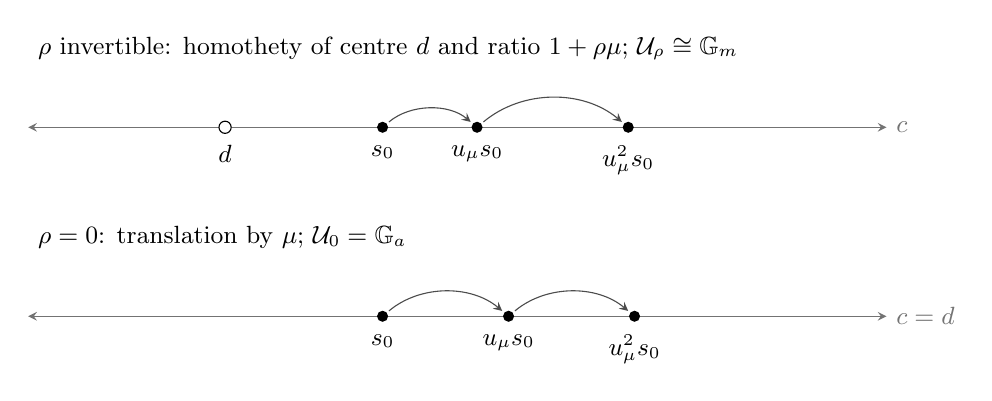
\begin{tikzpicture}[x=2cm, y=1cm, >=stealth, every node/.style={font=\small}]
\begin{scope}
\draw[black!55, <->] (-2.25,0) -- (3.2,0) node[right] {$c$};
\draw[fill=white] (-1,0) circle (2.2pt); \node[below=3pt] at (-1,0) {$d$};
\foreach \x/\l in {0/s_0, 0.6/u_\mu s_0, 1.56/u_\mu^2 s_0} { \fill (\x,0) circle (2pt); \node[below=3pt] at (\x,0) {$\l$}; }
\draw[->, black!70, shorten >=3pt, shorten <=3pt] (0,0) to[bend left=40] (0.6,0);
\draw[->, black!70, shorten >=3pt, shorten <=3pt] (0.6,0) to[bend left=40] (1.56,0);
\node[anchor=west] at (-2.25,1.0) {$\rho$ invertible: homothety of centre $d$ and ratio $1 + \rho\mu$; $\mathcal U_\rho \cong \mathbb G_m$};
\end{scope}
\begin{scope}[yshift=-2.4cm]
\draw[black!55, <->] (-2.25,0) -- (3.2,0) node[right] {$c = d$};
\foreach \x/\l in {0/s_0, 0.8/u_\mu s_0, 1.6/u_\mu^2 s_0} { \fill (\x,0) circle (2pt); \node[below=3pt] at (\x,0) {$\l$}; }
\draw[->, black!70, shorten >=3pt, shorten <=3pt] (0,0) to[bend left=40] (0.8,0);
\draw[->, black!70, shorten >=3pt, shorten <=3pt] (0.8,0) to[bend left=40] (1.6,0);
\node[anchor=west] at (-2.25,1.0) {$\rho = 0$: translation by $\mu$; $\mathcal U_0 = \mathbb G_a$};
\end{scope}
\end{tikzpicture}
\caption{The projective line $D_0$ of start vectors, in the chart $\langle s, a'_0\rangle = 1$, with the centre $c$ at infinity and $d$ the point where $\pi$ vanishes. Drawn for $\rho = 1$, $\mu = 0.6$, then $\rho = 0$, $\mu = 0.8$.}\label{fig:torsor}
\end{figure}

\subsection*{Invariant subspaces}
Over a field, with $h_i = ka_i$, $H_i = \ker a'_i$, $Z'_i = H_0 \cap \dots \cap H_i$, $Z^*_i = \langle h_{i+1}, \dots, h_n\rangle$ and $C$ the hyperplane $\pi = 0$:

\begin{theorem}[Grothendieck, \fac{72}, p.~79]\label{thm:inv}
Over a field, for arbitrary $\mu_i$ (characteristic $2$ included), a subspace of $E$ is stable under all the $\tau_i$ iff it is $0$, $E$, the line $k\tilde c$, the hyperplane $C$, or $Z'_i$ or $Z^*_i$ for some $i < n$ with $\beta_i = 0$.
\end{theorem}

\begin{corollary}[after \fac{72}, pp.~80--82]\label{cor:irr}
The representation on $C$ is irreducible iff all the $\beta_i$ are nonzero and, for $n \ge 1$, $\rho \ne 0$.
\end{corollary}

\begin{proof}
Intersect the list of Theorem~\ref{thm:inv} with $C$: $E \not\subset C$ since $\pi(s_0) = 1$; $k\tilde c \subset C$ iff $\rho = 0$; $Z^*_i \subset C$ always. If $\beta_i = 0$ for some $i < n$, then $Z^*_i$ is a stable subspace of $C$ that is neither $0$ nor $C$: it contains $h_{i+1}$ but not $h_0$, which lies in $C$. If $\rho = 0$ and $n \ge 1$, $k\tilde c$ is a line of $C$ different from $C$, since $h_0 \subset C$ is not a multiple of $\tilde c$, whose last coordinate is $1$.
\end{proof}

The struck-out (d) of page~80 asks for $\rho \ne 0$ and all $\beta_i \ne 0$; the (c) of page~82 omits $\rho \ne 0$, which is needed. For $i < n$, $Z^*_i \subset Z'_i$ iff $\beta_i = 0$, the ``$\in$'' of the margin of page~79 rather than the ``$\notin$'' of page~81.

\section{The icosahedron over \texorpdfstring{$\Z[\alpha]$}{Z[alpha]}}\label{sec:ico}

Section~VII of folder~70 writes the regular icosahedron over $\Z[\alpha] = \Z[x]/(x^2 + x - 1)$ by three reflections in the vertex frame $(s_0, s_1 - s_0, s_2 - s_0, s_3 - s_0)$ (pp.~74--75). Let $R$ be a commutative ring with $\alpha^2 + \alpha - 1 = 0$, put $\alpha' = -1 - \alpha$ (the other root), and
\[
\sigma_0(x,y,z) = \bigl(1 - (x+y+z), y, z\bigr),\quad \sigma_1(x,y,z) = (y + \alpha'z, x - \alpha'z, z),\quad \sigma_2(x,y,z) = (x, z, y),
\]
$\iota(x,y,z) = (\alpha' - x, 1 - \alpha' - y, 1 - \alpha' - z)$. The twelve vertices are $s_0 = 0$, $s_1 = e_1$, $s_2 = e_2$, $s_3 = e_3$, $s'_3 = (\alpha', -\alpha', 1)$, $s''_3 = (0, -\alpha', 1)$ and their images by $\iota$. Put
\[
q_0 = x^2 + y^2 + z^2 - \alpha yz + zx + xy, \qquad q = q_0 - (x + y + z).
\]
The thirty edges are the pairs of vertices at $q_0$-distance $1$ over $\Q(\sqrt5)$, and the twenty faces are the triangles of edges. A point $p$ is \emph{on the line} $(r, u)$ if $p - r = a(u - r)$ for some $a \in R$, and \emph{in the plane} $(r, u, w)$ if $p - r = s(u - r) + t(w - r)$; over a field these are collinearity and coplanarity.

\begin{theorem}[after \fac{70}, pp.~74--94]\label{thm:faithful}
Let $R$ be a nonzero commutative ring in which $\alpha^2 + \alpha = 1$.
\begin{enumerate}
\item The $\sigma_i$ permute the twelve vertices, by permutations of $\{0, \dots, 11\}$ independent of $R$; the vertices lie on $q = 0$, and $q_0(s' - s) = 1$ for each edge $\{s, s'\}$.
\item The twelve vertices are distinct; no three distinct vertices are collinear; and no vertex lies in the plane of a face not containing it.
\item The group $G$ generated by $\sigma_0, \sigma_1, \sigma_2$ has order $120$ and acts faithfully on the vertices.
\item If $2 = 0$ in $R$, $\iota$ is the translation by $(\alpha', \alpha, \alpha)$.
\end{enumerate}
\end{theorem}

\begin{proof}
(1) and (4) are polynomial identities modulo $\alpha^2 + \alpha - 1$. For (2), the $\sigma_i$ are affine, so a word in them transports equality of vertices, membership of a vertex in the line of two others, and in the plane of three others, along the corresponding permutation. Pages~93--94 invoke this homogeneity and treat only base cases; we make it explicit by two tables. For every ordered pair of distinct indices, a word sends it to $(s_0, s_1)$, $(s_0, s''_3)$ or $(s_0, \iota s_0)$; for every face, a word sends it to $(s_0, s_1, s_2)$. These $132 + 20$ facts concern permutations of twelve points and are checked by computation. In the base cases, $s_k$ is on the line $(s_0, s_j)$ only if the three $2 \times 2$ minors of $(s_k, s_j)$ vanish; for $j \in \{1, 5, 6\}$ and each of the thirty indices $k \ne 0, j$, one of them is a unit of $\Z[\alpha]$ ($\pm1$, $\pm(1+\alpha)$, $\pm(2+\alpha)$ or $\pm(3+2\alpha)$), which gives $1 = 0$. A vertex in the plane $z = 0$ of the face $(s_0, s_1, s_2)$ would have third coordinate $0$, whereas the nine other vertices have third coordinate $1$, $2 + \alpha$ or $1 + \alpha$, all units. For (3), a breadth-first enumeration gives $120$ words in the three permutations, closed under left multiplication by the generators; and an element of $G$ is affine and determined by the images of $s_0, \dots, s_3$, so $G$ is isomorphic to its permutation group.
\end{proof}

Ji \cite{ji2023} writes formulae over $\Z[\cos\theta, \cos\gamma]$ whose reduction is undefined at $2$ and $5$, shows that the automorphism group stays $A_5$ at the other primes, and notes that Grothendieck ``seems to claim this in all cases''. Theorem~\ref{thm:faithful} confirms the claim, for the incidences, in every characteristic, by the integral frame of the page. The proof needs no field and no norm computation beyond thirty invertible minors. The margin ``c'est en fait faux en car.~2~!'' therefore concerns neither the non-collinearity nor the face planes, and the translation vector of $\iota$ in characteristic~$2$ is $(\alpha', \alpha, \alpha)$, not the $(\alpha', 1, 1)$ read on page~91.

\begin{theorem}[Grothendieck, \fac{70}, pp.~101--106]\label{thm:quadric}
Let $R$ be a commutative ring with $\alpha^2 + \alpha = 1$.
\begin{enumerate}
\item $q$ is invariant under the $\sigma_i$, and every quadratic function vanishing at the nine vertices $s_0, s_1, s_2, s_3, s'_3, s''_3$, $\iota s_0, \iota s_1, \iota s_2$ is a multiple of $q$.
\item The half-discriminant of $q_0$ is $1$.
\item The projective quadric $Q = q_0(x,y,z) - (x+y+z)t$ has discriminant $-\alpha - 3$, of norm $5$. The discriminant is invertible iff $5$ is invertible in $R$, and then $0$ is the only common zero of the four partial derivatives of $Q$: $Q$ is smooth.
\item If $5 = 0$ and $\alpha = 2$, $Q$ is a cone with vertex the centre $o = (1, 2, 2)$. Over a field, $Q$ is singular iff the characteristic is $5$.
\end{enumerate}
\end{theorem}

\begin{proof}
The uniqueness follows from a $9 \times 9$ minor equal to $13\alpha + 21$, a unit of $\Z[\alpha]$ with inverse $13\alpha - 8$; it holds over any ring, without dividing. The half-discriminant $4abc + uvw - au^2 - bv^2 - cw^2$ of $q_0$ is $2 - (\alpha^2 + \alpha) = 1$, the \emph{merveille} of page~101, also in characteristic~$2$. The $4 \times 4$ polar matrix of $Q$ has determinant $\alpha^2 - 4 = -\alpha - 3$; since $(-\alpha - 3)(\alpha - 2) = 5$ and $(-\alpha - 3)^2 = 5(\alpha + 2)$, it is invertible iff $5$ is. The rows of the polar matrix are the partial derivatives of $Q$, and a square matrix with invertible determinant has zero kernel. In characteristic $5$, $\alpha^2 + \alpha - 1 = (\alpha - 2)^2$, and the kernel is spanned by $(1, 2, 2, 1)$, which lies on $Q$.
\end{proof}

\begin{theorem}[after \fac{70}, p.~78]\label{thm:mod5}
Over $\F_5$, where $\alpha = 2$, put $\bar s = s - o$ for a vertex $s$.
\begin{enumerate}
\item The twelve $\bar s$ are isotropic for $q_0$, and the nonzero isotropic vectors of $q_0$ are exactly the twelve $\bar s$ and their doubles $2\bar s$, twenty-four distinct vectors.
\item A point of $\mathbb P^2(\F_5)$ lies on the conic $q_0 = 0$ iff it is one of the six vertex directions.
\item The six vertex directions, fifteen edge directions $s' - s$ and ten face directions $\bar a + \bar b + \bar c$ are the $31 = 5^2 + 5 + 1$ points of $\mathbb P^2(\F_5)$, each once.
\item A face direction is $q_0$-orthogonal to the plane of its face. Through an edge direction pass exactly two tangents to the conic, through a face direction none; $q_0$ takes the values $1$ or $4$ on $60$ vectors and $2$ or $3$ on $40$, so that $125 = 1 + 24 + 60 + 40$.
\end{enumerate}
\end{theorem}

\begin{proof}
All statements concern the $125$ vectors of $\F_5^3$ and finite lists of vertices, edges and faces, and are checked by computation.
\end{proof}

Page~78 gives the table of directions, the count $125 = 1 + 24 + 60 + 40$, and the phrase ``deux icos.'': the twenty-four isotropic vectors are the vertices of the icosahedron and of its homothetic image of ratio~$2$. Points~(2) and~(4) explain the fifteen edge directions as the exterior points of the conic and the ten face directions as the interior points (Figure~\ref{fig:conic}); that $\mathfrak A_5 \cong \mathrm{PSL}_2(\F_5)$ acts on the six axes as on $\mathbb P^1(\F_5)$ is classical, but we do not know a printed source that reads the reduction modulo~$5$ of the icosahedron as this conic and its exterior and interior points. This is one of the two most singular characteristics of the \emph{Esquisse}: the quadric degenerates to a cone, and the icosahedron survives on its isotropic directions. A footnote of the \emph{Esquisse} suggests that the exceptional characteristics are those where the circumscribed hyperquadric is degenerate or tangent to the hyperplane at infinity \cite[\S4]{esquisse}. Characteristic $5$ is the degenerate case. In characteristic $2$ the conic at infinity $q_0 = 0$ stays smooth, since its half-discriminant is $1$; what happens there is that the centre goes to infinity, as the \emph{Esquisse} says of characteristic~$2$: by Theorem~\ref{thm:faithful}(4), $\iota$ is a translation.

\begin{figure}[ht]
\centering
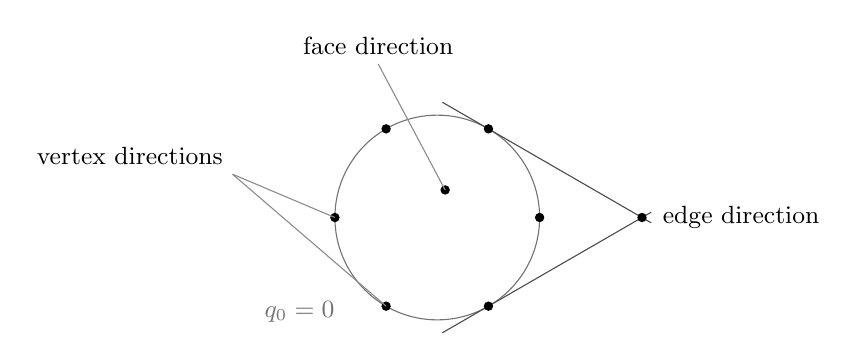
\begin{tikzpicture}[x=1cm, y=1cm, every node/.style={font=\small}]
\draw[black!55] (0,0) circle (1.3);
\coordinate (E) at (2.6,0);
\draw[black!70] ($(E)!-0.06!(60:1.3)$) -- ($(E)!1.3!(60:1.3)$);
\draw[black!70] ($(E)!-0.06!(-60:1.3)$) -- ($(E)!1.3!(-60:1.3)$);
\foreach \a in {0,60,...,300} \fill (\a:1.3) circle (1.7pt);
\fill (E) circle (1.7pt); \node[right=4pt] at (E) {edge direction};
\fill (0.1,0.35) circle (1.7pt); \draw[black!45] (0.1,0.35) -- (-0.75,1.95); \node[anchor=south] at (-0.75,1.95) {face direction};
\draw[black!45] (180:1.3) -- (-2.6,0.55); \draw[black!45] (240:1.3) -- (-2.6,0.55); \node[anchor=south east] at (-2.6,0.55) {vertex directions};
\node[black!55] at (-1.75,-1.2) {$q_0 = 0$};
\end{tikzpicture}
\caption{Theorem~\ref{thm:mod5}, drawn schematically over $\R$. In $\mathbb P^2(\F_5)$ the conic $q_0 = 0$ consists of the six vertex directions; each of the fifteen edge directions lies on exactly two tangents, and none of the ten face directions lies on a tangent.}\label{fig:conic}
\end{figure}

\section{The combinatorial icosahedron and the hemi-icosahedron}\label{sec:comb}

Folder~86 takes the icosahedron as a purely combinatorial object. Label its vertices $0, \dots, 11$, with $0$ and $11$ opposite and $1, \dots, 5$ and $6, \dots, 10$ the two pentagons of their neighbours; everything below is computed from the adjacency. For a face $\{x, y, z\}$, let $\mathrm o(x, y, z)$ be the third vertex of the other face bordering $\{x, y\}$, and let $\iota x$ be the antipode, the only vertex that is neither $x$ nor a neighbour of $x$ nor a neighbour of a neighbour. A \emph{flag} is an oriented triangle $(s, t, u)$; there are $120$. Figure~\ref{fig:triedre} shows the labelling. Two edges have the same \emph{direction} if they are equal or antipodal. For an edge $\{s, t\}$ with faces $\{s, t, u\}$, $\{s, t, v\}$, page~18 defines $\rho_0(s, t) = \{\mathrm o(s, u, t), \mathrm o(s, v, t)\}$: the side of the pentagon around $s$ opposite to $t$ (Figure~\ref{fig:rho0}).

\begin{figure}[ht]
\centering
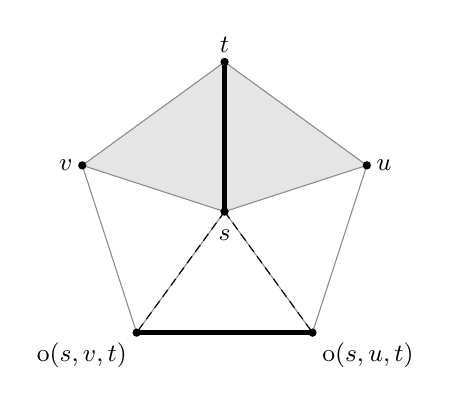
\begin{tikzpicture}[x=1cm, y=1cm, every node/.style={font=\small}]
\coordinate (s) at (0,0);
\coordinate (t) at (90:1.9); \coordinate (u) at (18:1.9); \coordinate (a) at (-54:1.9);
\coordinate (b) at (-126:1.9); \coordinate (v) at (162:1.9);
\fill[black!10] (s)--(t)--(u)--cycle; \fill[black!10] (s)--(t)--(v)--cycle;
\draw[black!45] (t)--(u)--(a)--(b)--(v)--cycle;
\foreach \p in {u,a,b,v} \draw[black!45] (s)--(\p);
\draw[densely dashed] (s)--(a); \draw[densely dashed] (s)--(b);
\draw[line width=1.6pt] (s)--(t);
\draw[line width=1.6pt] (a)--(b);
\foreach \p in {s,t,u,a,b,v} \fill (\p) circle (1.5pt);
\node[below=3pt] at (s) {$s$}; \node[above] at (t) {$t$}; \node[right] at (u) {$u$};
\node[left] at (v) {$v$};
\node[below right] at (a) {$\mathrm o(s, u, t)$}; \node[below left] at (b) {$\mathrm o(s, v, t)$};
\end{tikzpicture}
\caption{The construction of page~18 at a vertex $s$, whose five neighbours form a pentagon. The edge $\{s, t\}$ (thick) borders the faces $\{s, t, u\}$ and $\{s, t, v\}$ (grey). Across $\{s, u\}$ the other face is $\{s, u, \mathrm o(s, u, t)\}$, and likewise across $\{s, v\}$; the two vertices so reached span the side of the pentagon opposite to $t$ (thick), which is $\rho_0(s, t)$.}\label{fig:rho0}
\end{figure}

\begin{theorem}[Grothendieck, \fac{86}, pp.~18--25]\label{thm:triedres}
\leavevmode
\begin{enumerate}
\item $\rho_0$ induces a well-defined fixed-point-free permutation $\rho$ of the fifteen edge directions with $\rho^3 = \id$. Its five orbits, the \emph{distinguished trihedra}, each partition the twelve vertices into six edges, and at every vertex the five edges lie in the five different trihedra.
\item The automorphism group $G$ of the icosahedron has order $120$, commutes with $\iota$ and $\rho$, and acts on the set $T$ of the five trihedra through a homomorphism $G \to \mathfrak S_T$ with image $\Alt_T$ and kernel $\{1, \iota\}$.
\end{enumerate}
\end{theorem}

\begin{proof}
An automorphism commutes with $\mathrm o$, since $\mathrm o(x, y, z)$ is the only common neighbour of $x$ and $y$ other than $z$, and the twelve vertices are obtained from $0, 1, 2$ by nine applications of $\mathrm o$; so an automorphism is determined by the image of the flag $(0, 1, 2)$, and every flag is such an image. $\iota$ and $\rho$ are defined by adjacency, hence commute with $G$. The rest is a computation on the $120$ flags: the induced permutations of $T$ are even, there are $60$ of them, and only $(0,1,2)$ and $(\iota0, \iota1, \iota2)$ give the identity.
\end{proof}

Page~23 puts two edges of different trihedra in the same triple; the correction is part of the proof's check. The page's own argument goes through the parity of the generators and the orders $6$, $10$ and $4$ of the images of the stabilisers of a face, a vertex and an edge; here the statement is obtained by counting flags. In Euclidean terms the trihedra are the five orthogonal frames, or the five octahedra inscribed in the icosahedron; that identification is not used.

\begin{figure}[ht]
\centering
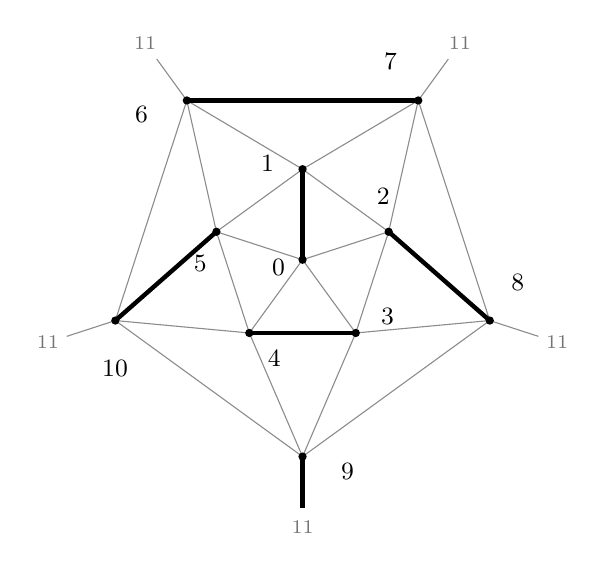
\begin{tikzpicture}[x=1cm, y=1cm, every node/.style={font=\small}]
\coordinate (v0) at (0,0);
\foreach \k in {1,...,5} { \coordinate (v\k) at ({90-72*(\k-1)}:1.15); }
\coordinate (v7) at (54:2.5); \coordinate (v8) at (-18:2.5); \coordinate (v9) at (-90:2.5);
\coordinate (v10) at (-162:2.5); \coordinate (v6) at (126:2.5);
\foreach \a/\b in {0/1,0/2,0/3,0/4,0/5,1/2,2/3,3/4,4/5,5/1,1/6,1/7,2/7,2/8,3/8,3/9,4/9,4/10,5/10,5/6,6/7,7/8,8/9,9/10,10/6} \draw[black!45] (v\a)--(v\b);
\foreach \k/\ang in {7/54,8/-18,9/-90,10/-162,6/126} { \draw[black!45] (v\k)--(\ang:3.15); \node[black!55, font=\scriptsize] at (\ang:3.4) {$11$}; }
\foreach \a/\b in {0/1,3/4,6/7,2/8,5/10} \draw[line width=1.6pt] (v\a)--(v\b);
\draw[line width=1.6pt] (v9)--(-90:3.15);
\foreach \k in {0,...,10} \fill (v\k) circle (1.5pt);
\node at (198:0.32) {$0$};
\foreach \k in {1,...,5} { \node at ({90-72*(\k-1)+20}:1.3) {$\k$}; }
\foreach \k/\ang in {7/54,8/-18,9/-90,10/-162,6/126} { \node at (\ang+12:2.75) {$\k$}; }
\end{tikzpicture}
\caption{The icosahedron of Section~\ref{sec:comb}, projected from the vertex $11$: $0$ at the centre, the pentagons $1, \dots, 5$ and $6, \dots, 10$ around it, and $11$ at infinity, joined to $6, \dots, 10$ by the radial segments. In thick lines, one of the five distinguished trihedra: the six edges $\{0,1\}$, $\{9,11\}$, $\{3,4\}$, $\{6,7\}$, $\{2,8\}$, $\{5,10\}$, pairwise disjoint, in three directions of two antipodal edges each.}\label{fig:triedre}
\end{figure}

\begin{theorem}[after \fac{86}, pp.~21, 26--32]\label{thm:hemi}
To a flag $(s, t, u)$, with $v = \mathrm o(s, t, u)$, associate the numbering $\nu(s, t, u)\colon \{1, \dots, 5\} \to T$ formed by the trihedra of the five edges at $s$, read around the pentagon from $t$, away from $u$.
\begin{enumerate}
\item All the $\nu(s, t, u)$ have the same parity; they define an orientation $\varpi$ of $T$ independent of all choices. Every numbering compatible with $\varpi$ is some $\nu(s, t, u)$, and $\nu(s, t, u) = \nu(s', t', u')$ iff the flags are equal or antipodal. The $60$ flags of the hemi-icosahedron $\bar\Pi = \Pi/\iota$ are thus the $60$ numberings of $T$ compatible with $\varpi$.
\item Changing the vertex, the edge or the face of a flag composes $\nu$ on the right with $\tau_0 = (2\,4)(3\,5)$, $\tau_1 = (1\,5)(2\,4)$, $\tau_2 = (2\,5)(3\,4)$.
\item Two flags of $\bar\Pi$ have the same vertex iff their numberings trace the same pentagon on $T$, the same edge iff they give the same partition $\{a_1\} \sqcup \{a_2, a_3\} \sqcup \{a_4, a_5\}$, and the same face iff they give the same three-element set $\{a_1, a_3, a_5\}$. One obtains $6$ pentagons, all $15$ partitions of type $(2,2,1)$, and the $10$ three-element subsets of $T$.
\end{enumerate}
\end{theorem}

\begin{proof}
By Theorem~\ref{thm:triedres}, $\nu(g0, g1, g2)$ is the permutation of $T$ induced by $g$, composed with $\nu(0, 1, 2)$, which is even with our labelling; surjectivity onto $\Alt_T$ and the kernel $\{1, \iota\}$ give (1). The changes of flag are right multiplications by three fixed automorphisms, and (2) reduces to three equalities of permutations. For (3), one reduces by an automorphism to the flag $(0, 1, 2)$ and checks the $120$ flags; the ten symmetries of the pentagon $1\,2\,3\,4\,5$ are even permutations of the places, which is why a numbering traces the pentagon of a vertex iff it is compatible with $\varpi$.
\end{proof}

The hemi-icosahedron has six vertices, fifteen edges and ten faces, its skeleton is $K_6$ and its group is $\Alt_5$. The theorem rebuilds it from an oriented set of five points alone: vertices are the six pentagons compatible with the orientation, edges the fifteen partitions of type $(2,2,1)$, faces the ten three-element subsets. Pages~31--32 give the three involutions on numberings with a $\sigma_1$ that is $\tau_2\tau_1\tau_2$, conjugate to the one above; the two triples define isomorphic sets with operators.

\section{Verification}\label{sec:lean}
\begingroup\sloppy

Every theorem above is formalised in Lean~4 with Mathlib, in the files \texttt{Folder70.lean}, \texttt{Folder72.lean}, \texttt{Folder78.lean} and \texttt{Folder86.lean} of the repository \href{https://github.com/Commutator-IO/grothendieck-project}{Commutator-IO/grothendieck-project} (directory \texttt{lean/Grothendieck}); the proofs use only Lean's standard axioms, and the finite statements (the words of Theorem~\ref{thm:faithful}, the computations over $\F_5$, the $120$ flags of Section~\ref{sec:comb}) are checked by the kernel. The main declarations are \texttt{F\_bezout}, \texttt{u\_zpow\_apply}, \texttt{zpow\_eq\_one\_iff}, \texttt{strip\_vertex} and \texttt{strip\_lines} in \texttt{Folder78}; \texttt{orderOf\_rho\_eq\_three}, \texttt{orderOf\_rho\_eq\_four}, \texttt{orderOf\_rho\_eq\_five}, \texttt{orderOf\_rho\_eq\_iff}, \texttt{not\_collinear\_any}, \texttt{not\_in\_face\_plane\_any}, \texttt{card\_icoGroup}, \texttt{quadric\_unique}, \texttt{qHom\_smooth} and \texttt{conic\_iff} in \texttt{Folder70}; \texttt{condAs\_iff\_condBs}, \texttt{pinned\_classification}, \texttt{centraliserEquiv}, \texttt{invariant\_iff} and \texttt{irreducible\_on\_C\_iff} in \texttt{Folder72}; \texttt{rho\_cube}, \texttt{permT\_surjective}, \texttt{permT\_eq\_one\_iff}, \texttt{numb\_eq\_iff}, \texttt{incidence\_dictionary} and \texttt{counts} in \texttt{Folder86}. These files are also part of the Palomar Registry repository \href{https://github.com/Commutator-IO/grothendieck-project-palomar}{Commutator-IO/grothendieck-project-palomar}.

\endgroup

Not proved here: the passage from the definition of a regular realisation to the normal form of pages~7--18 of folder~70; the order criterion for arbitrary $p$ in positive characteristic; the identification of $G$ with the Coxeter group $H_3 \cong \mathfrak A_5 \times \Z/2$; the scheme $\mathcal U_\rho$ and the projective statement of folder~72 over a base; the uniqueness, suggested in the reading of folder~78, of the improper $2p$-gon among non-unimodular regular polygons.

\section*{Statement on the use of artificial intelligence}
The transcriptions of folders~70, 72, 78 and~86, the modernised readings, the proofs, the Lean formalisation and a first draft of this text were produced with language models (Claude Opus~5 and Opus~5.5, Anthropic), under the author's direction. The author checked the statements, the proofs and the references, and takes full responsibility for the content. The formal proofs are checked mechanically by Lean.

\section*{Acknowledgements}
The facsimiles are published by the University of Montpellier, \href{https://grothendieck.umontpellier.fr/}{grothendieck.umontpellier.fr}.

\begin{thebibliography}{10}
\bibitem{coxeter1973} H.~S.~M.~Coxeter, \emph{Regular Polytopes}, 3rd ed., Dover, New York, 1973.
\bibitem{dgklm2021} J.~Danciger, F.~Guéritaud, F.~Kassel, G.-S.~Lee, L.~Marquis, Convex cocompactness for Coxeter groups, \emph{J. Eur. Math. Soc.} 27 (2025), no.~1, 119--181, \href{https://doi.org/10.4171/jems/1539}{doi:10.4171/jems/1539}; section numbers as in arXiv:2102.02757v3.
\bibitem{esquisse} A.~Grothendieck, Esquisse d'un programme, in L.~Schneps, P.~Lochak (eds.), \emph{Geometric Galois Actions 1}, London Math.\ Soc.\ Lecture Note Ser.~242, Cambridge University Press, 1997, 7--48, \href{https://doi.org/10.1017/CBO9780511758874.003}{doi:10.1017/CBO9780511758874.003}; English translation by P.~Lochak and L.~Schneps, Sketch of a Programme, ibid., 243--283, \href{https://doi.org/10.1017/CBO9780511758874.017}{doi:10.1017/CBO9780511758874.017}.
\bibitem{fisherjamison1998} J.~C.~Fisher, R.~E.~Jamison, Properties of affinely regular polygons, \emph{Geom.\ Dedicata} 69 (1998), 241--259, \href{https://doi.org/10.1023/A:1004903818702}{doi:10.1023/A:1004903818702}.
\bibitem{ji2023} C.~Ji, A note on regular polyhedra over finite fields, arXiv:2304.03345 (2023).
\bibitem{korchmarosszonyi2008} G.~Korchmáros, T.~Sz\H{o}nyi, Affinely regular polygons in an affine plane, \emph{Contrib.\ Discrete Math.} 3 (2008), no.~1, 20--38, \href{https://doi.org/10.55016/ojs/cdm.v3i1.62767}{doi:10.55016/ojs/cdm.v3i1.62767}.
\bibitem{lucas1878} É.~Lucas, Théorie des fonctions numériques simplement périodiques, \emph{Amer.\ J.\ Math.} 1 (1878), no.~2, 184--196; no.~3, 197--240; no.~4, 289--321, \href{https://doi.org/10.2307/2369308}{doi:10.2307/2369308}, \href{https://doi.org/10.2307/2369311}{10.2307/2369311}, \href{https://doi.org/10.2307/2369373}{10.2307/2369373}.
\bibitem{mcmullenschulte2002} P.~McMullen, E.~Schulte, \emph{Abstract Regular Polytopes}, Cambridge University Press, 2002, \href{https://doi.org/10.1017/CBO9780511546686}{doi:10.1017/CBO9780511546686}.
\bibitem{monsonschulte2004} B.~Monson, E.~Schulte, Reflection groups and polytopes over finite fields, I, \emph{Adv.\ Appl.\ Math.} 33 (2004), 290--317, \href{https://doi.org/10.1016/j.aam.2003.11.002}{doi:10.1016/j.aam.2003.11.002}.
\end{thebibliography}

\end{document}
